\documentclass[10pt,a4paper]{article}
\usepackage[T1]{fontenc}
\usepackage[utf8]{inputenc}
\usepackage[french]{babel}
\usepackage[margin=1.5cm]{geometry}
\usepackage{helvet}\renewcommand{\familydefault}{\sfdefault}
\usepackage{xcolor}
\definecolor{btkblue}{HTML}{14507A}
\definecolor{btkcyan}{HTML}{00AEEF}
\definecolor{btklight}{HTML}{EAF3FA}
\definecolor{ink}{HTML}{233140}
\color{ink}
\usepackage{titlesec}
\usepackage{enumitem}
\usepackage{pifont}
\setlist[itemize]{leftmargin=1.25em,itemsep=1.5pt,topsep=2pt,parsep=0pt}
\usepackage{graphicx}
\usepackage[most]{tcolorbox}
\usepackage{multicol}
\usepackage[hidelinks]{hyperref}

\titleformat{\section}{\large\bfseries\color{btkblue}}{}{0pt}{}
\titlespacing{\section}{0pt}{7pt}{2pt}
\newcommand{\rulecyan}{\par\vspace{-3pt}\textcolor{btkcyan}{\rule{\linewidth}{1pt}}\par\vspace{2pt}}
\pagestyle{empty}
\setlength{\parindent}{0pt}

\begin{document}

% ---------- HEADER ----------
\noindent
\begin{minipage}[c]{0.30\textwidth}
\includegraphics[width=3.1cm]{logo_esb.png}\end{minipage}
\hfill
\begin{minipage}[c]{0.38\textwidth}\centering
{\footnotesize Esprit School of Business\\ Licence Business Computing --- Parcours \textbf{Business Intelligence}}
\end{minipage}
\hfill
\begin{minipage}[c]{0.18\textwidth}\raggedleft
\includegraphics[width=1.7cm]{logo_btk.png}\end{minipage}

\vspace{6pt}
\begin{tcolorbox}[colback=btkblue,colframe=btkblue,boxrule=0pt,arc=2pt,
  left=12pt,right=12pt,top=8pt,bottom=8pt]
\color{white}
{\large\bfseries PROJET DE FIN D'ÉTUDES --- Fiche de présentation}\\[3pt]
{\normalsize Conception et développement d'un \textbf{système intelligent de gestion
des rôles et de pointage des employés} avec \textbf{tableau de bord décisionnel}}
\end{tcolorbox}

\vspace{3pt}
{\footnotesize
\textbf{Étudiant :} Oussema Korbosli \;\textbar\; \textbf{Encadrant académique :} Heni Abidi
\;\textbar\; \textbf{Maître de stage :} Melek Aziz Elmoula (Data Scientist)\\
\textbf{Organisme :} BTK --- Banque Tuniso-Koweïtienne \;\textbar\;
\textbf{Période :} 16/02/2026 -- 16/06/2026}

\vspace{4pt}
\begin{tcolorbox}[colback=btklight,colframe=btkcyan,boxrule=1pt,arc=2pt,
  left=8pt,right=8pt,top=5pt,bottom=5pt]
\textbf{En une phrase.} Une application web \textbf{Jakarta EE / Oracle} qui
centralise la gestion du réseau d'agences de la BTK (agences, employés, clients,
objectifs), gère les \textbf{rôles} et la sécurité, assure le \textbf{pointage de
présence} des employés, et restitue les indicateurs clés via \textbf{Power BI} et
un tableau de bord embarqué.
\end{tcolorbox}

% ---------- BODY ----------
\section{Contexte \& problématique}\rulecyan
La BTK gère un large réseau d'agences (\textasciitilde 45 agences,
\textasciitilde 400 collaborateurs). La gestion actuelle est \textbf{dispersée}
(fichiers non centralisés), \textbf{sans pointage formalisé}, avec une faible
traçabilité et peu d'indicateurs de pilotage.\\
\textit{Problématique :} comment \textbf{centraliser et fiabiliser} la gestion du
réseau, \textbf{encadrer} les opérations sensibles, \textbf{suivre la présence}
des employés et \textbf{exploiter les données} pour la décision ?

\section{Objectifs}\rulecyan
\begin{itemize}
  \item Gérer les utilisateurs et les \textbf{rôles} ; renforcer la \textbf{sécurité} des accès.
  \item \textbf{Centraliser} les données du réseau (agences, employés, clients, objectifs).
  \item \textbf{Assurer le pointage} (présence) des employés.
  \item Développer un \textbf{tableau de bord décisionnel} (BI).
\end{itemize}

\begin{multicols}{2}
\section{Architecture}\rulecyan
\textbf{Logique (MVC, en couches) :}
\begin{itemize}
  \item Présentation : JSP / JSTL, CSS, ApexCharts
  \item Contrôle : Servlets \texttt{@WebServlet} + filtre
  \item Métier : services \textbf{EJB}
  \item Persistance : \textbf{JPA / Hibernate} $\rightarrow$ Oracle
\end{itemize}
\textbf{Physique (3-tiers) :} navigateur $\rightarrow$ serveur \textbf{WildFly}
(WAR) $\rightarrow$ serveur \textbf{Oracle} ; poste \textbf{Power BI} connecté aux
vues décisionnelles.

\columnbreak
\begin{center}
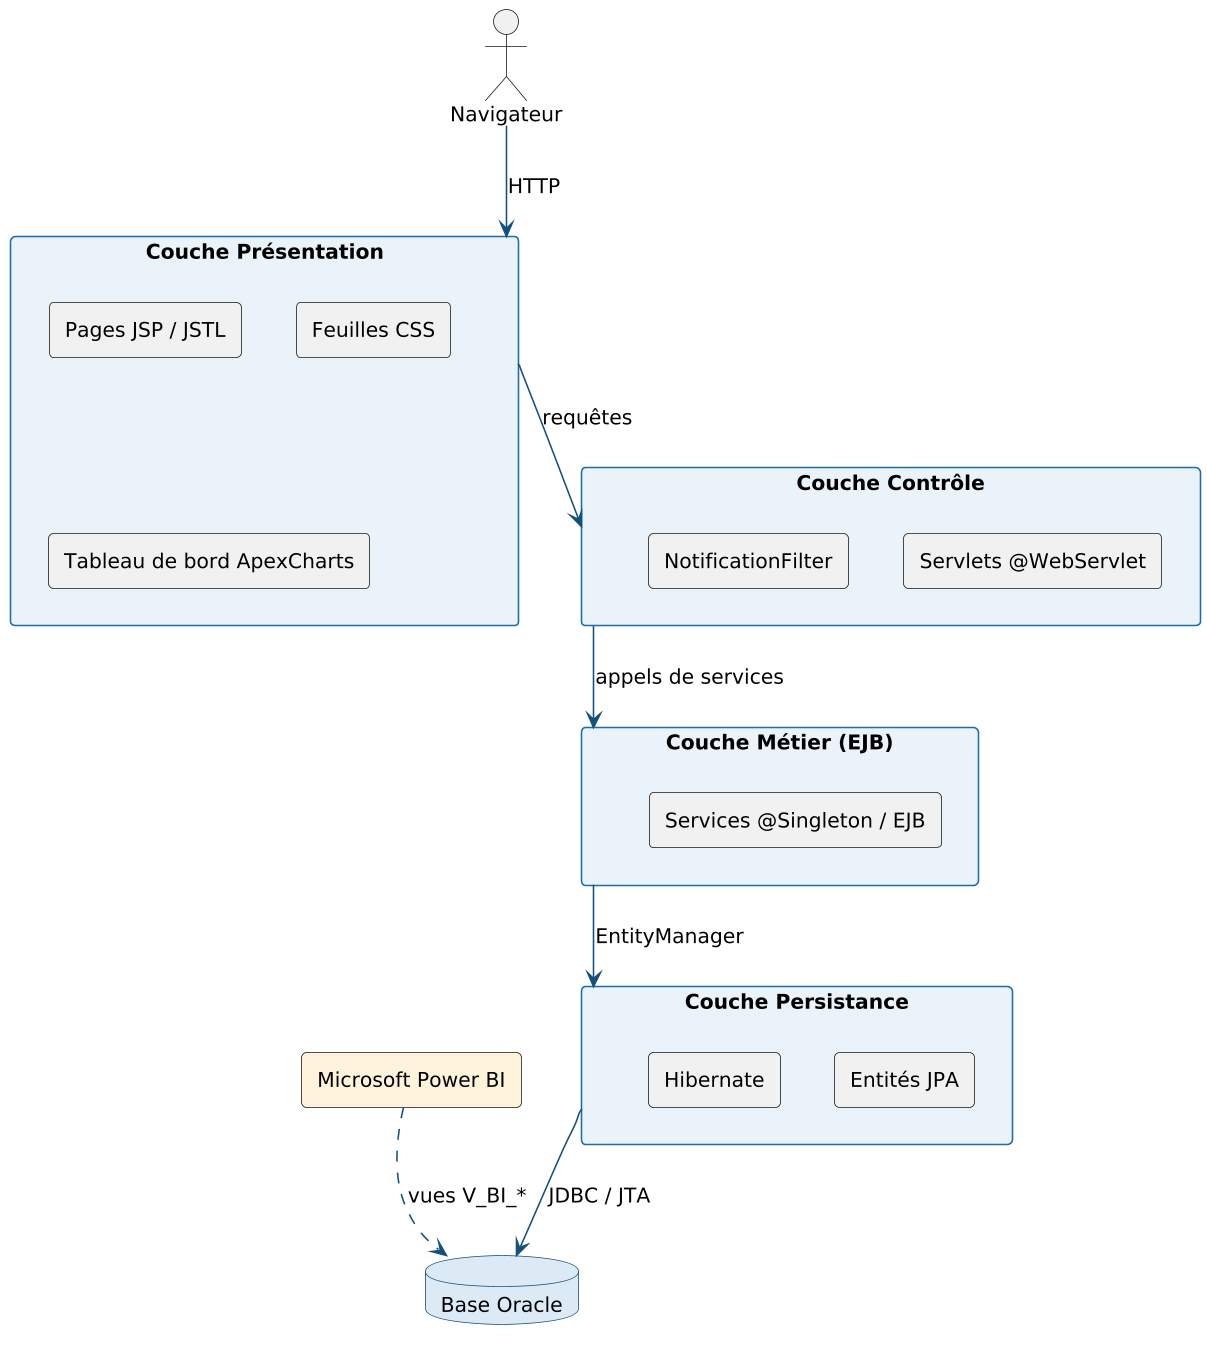
\includegraphics[width=4.7cm]{archi_logique.png}\\
{\footnotesize\color{btkblue}\textbf{Architecture logique en couches}}
\end{center}
\end{multicols}

\section{Modules fonctionnels}\rulecyan
\begin{multicols}{2}
\begin{itemize}
  \item Authentification \& gestion des \textbf{rôles} (ADMIN, DIRECTEUR, USER)
  \item Gestion des \textbf{agences} / \textbf{employés}
  \item Gestion des \textbf{clients} / \textbf{objectifs}
  \item \textbf{Pointage} (arrivée/départ, statut, auto + manuel)
  \item \textbf{Workflow de demandes} (validation par l'admin)
  \item \textbf{Tableau de bord}, notifications, journal d'audit
\end{itemize}
\end{multicols}

\section{Volet décisionnel (Business Intelligence)}\rulecyan
Vues analytiques Oracle \texttt{V\_BI\_EMPLOYES}, \texttt{V\_BI\_CLIENTS},
\texttt{V\_BI\_OBJECTIFS}, \texttt{V\_BI\_POINTAGE} (\textbf{modèle en étoile} :
faits + dimensions agence/période). Consommées par \textbf{Power BI} et un
\textbf{tableau de bord embarqué} (ApexCharts) : KPI (effectifs, \textbf{taux de
présence}, demandes), effectif par agence, répartition des rôles, présence du jour.

\begin{multicols}{2}
\section{Technologies}\rulecyan
Java 21 \textbar{} \textbf{Jakarta EE 10} (Servlets, JSP/JSTL, EJB, JPA) \textbar{}
Hibernate \textbar{} \textbf{Oracle} \textbar{} \textbf{WildFly} \textbar{} Maven
\textbar{} \textbf{Power BI} / ApexCharts \textbar{} Git/GitHub.

\section{Méthodologie}\rulecyan
\textbf{Scrum} : sprints successifs (cadrage $\rightarrow$ sécurité $\rightarrow$
agences/employés $\rightarrow$ clients/objectifs $\rightarrow$ \textbf{pointage}
$\rightarrow$ BI $\rightarrow$ tests/rédaction).
\end{multicols}

\section{Conception (UML)}\rulecyan
Cas d'utilisation \textbar{} \textbf{Classes} (entités JPA, associations réelles,
sans héritage inventé) \textbar{} \textbf{Séquences} (authentification, validation
de demande, pointage) \textbar{} \textbf{Activité} \textbar{} \textbf{États-transitions}
\textbar{} Architecture \textbf{logique} + \textbf{physique} \textbar{} \textbf{ER}
\textbar{} Modèle \textbf{BI en étoile} \textbar{} Gantt.

\begin{multicols}{2}
\section{État d'avancement}\rulecyan
\begin{itemize}
  \item[\textcolor{btkcyan}{\ding{52}}] Application \textbf{fonctionnelle, déployée et opérationnelle} (WildFly).
  \item[\textcolor{btkcyan}{\ding{52}}] Module \textbf{pointage} développé et intégré au BI/dashboard.
  \item[\textcolor{btkcyan}{\ding{52}}] \textbf{Tableau de bord professionnel} (KPI + graphiques).
  \item[\textcolor{btkcyan}{\ding{52}}] \textbf{Rapport (34 p.)} conforme à la charte ; code sur GitHub.
\end{itemize}

\section{Perspectives}\rulecyan
\begin{itemize}
  \item Hachage des mots de passe ; renforcement sécurité.
  \item Entrepôt de données / \textbf{ETL} (historisation).
  \item \textbf{Analyses prédictives} ; API REST ; app mobile.
\end{itemize}
\end{multicols}

\begin{tcolorbox}[colback=btklight,colframe=btkblue,boxrule=1pt,arc=2pt,
  left=8pt,right=8pt,top=5pt,bottom=5pt,
  title=\textbf{Questions probables de l'encadrant \textrightarrow{} réponses prêtes},
  coltitle=white,colbacktitle=btkblue]
\footnotesize
\textbf{Valeur ajoutée BI ?} Vues \texttt{V\_BI\_*} (étoile) + Power BI + dashboard
temps réel, dont le \textbf{taux de présence} issu du pointage.\\
\textbf{Pourquoi Jakarta EE ?} Standard d'entreprise : conteneur EJB + JTA + JPA,
robuste, adapté au secteur bancaire.\\
\textbf{Modèle de données ?} Entité centrale \texttt{Utilisateur} ; associations par
clés étrangères / \texttt{@ManyToOne} (agences, objectifs, demandes, pointage) ;
\textbf{pas d'héritage} (fidèle au code réel).\\
\textbf{Sécurité ?} Rôles + workflows de validation + journal d'audit ; amélioration
prévue : \textbf{hachage des mots de passe}.
\end{tcolorbox}

\end{document}
